% Nome do capítulo
\chapter{Segundo capítulo de exemplo}
% Label para referenciar
\label{cap2}

% Diminuir espaçamento entre título e texto
\vspace{-1.9cm}

% Texto do capítulo
  
  As figuras devem ser apresentadas pelos comandos abaixo. O parâmetro \textit{width} determina o tamanho que a figura
  será exibida. No parâmetro \textit{caption} o texto que aparece entre colchetes será o exibido no índice de figuras e o texto
  contido entre chaves será exibido na legenda da figura. Para citar a figura o comando ref deve ser usado juntamente
  com o label, como é mostrado nesse exemplo da Figura \ref{fig:ComponentesWiNoC}.

  \begin{figure}[H]
  % Alterar espaçamentos antes e depois do caption
  \setlength{\abovecaptionskip}{0pt}
  \setlength{\belowcaptionskip}{0pt}
  % Caption
  \caption[Principais componentes de WiNoCs]{Principais componentes de WiNoCs}
  \centering
  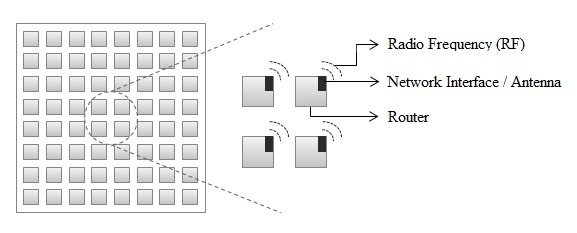
\includegraphics[width=.85\textwidth]{imagem/winoc.jpg}
  % Caption centralizada
  \captionsetup{justification=centering}
  \captionfont{\small{\textbf{\\Fonte: \cite{OliveiraIadis:2011}}}}	
  \label{fig:ComponentesWiNoC}
  \end{figure}


  Os comandos abaixo são usados para apresentação de gráficos. A diferença está apenas na definição do tipo ``grafico`` 
  que permite a adição dos itens no índice de gráficos de forma automática. Os parâmetros são semelhantes aos usados para
  representação de figuras. O parâmetro \textit{width} determina o tamanho do gráfico. O texto entre colchetes 
  no \textit{caption} será o exibido no índice de gráficos e o texto contido entre chaves será exibido na legenda.

\begin{grafico}[H]
  % Alterar espaçamentos antes e depois do caption
  \setlength{\abovecaptionskip}{5pt}
  \setlength{\belowcaptionskip}{0pt}
  % Caption
  \caption[Percentual de pacotes enviados]
	  {Percentual de pacotes enviados}
  \centering
  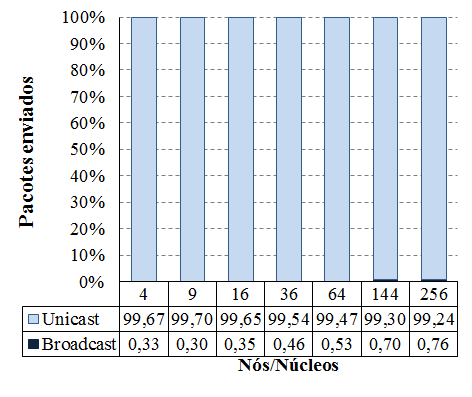
\includegraphics[width=.48\textwidth]{imagem/graficos/grafico_pacotes_enviados_bt.png}
  % Caption centralizada
  \captionsetup[grafico]{justification=centering}
  % Fonte
  \captionfont{\small{\textbf{\\Fonte: Dados da pesquisa}}}
  \end{grafico}

  

Um exemplo de criação de tabela é mostrado a seguir. As colunas são separadas por elementos \& e as linhas por duas barras invertidas. 
  Os comandos \textit{hline} e | definem a criação de linhas e colunas para separar os conteúdos, respectivamente. A tabela pode
  ser referenciada usando o comando ref juntamente com o label, como na Tabela \ref{tab:classesNas}. 

   % Tabela
  \begin{table}[H]
    \centering
    \footnotesize
    % Alterar espaçamentos antes e depois do caption
    \setlength{\abovecaptionskip}{0pt}
    \setlength{\belowcaptionskip}{0pt}
    % Caption
    \caption[Parâmetros definidos por classe]{Parâmetros definidos por classe}
    \label{tab:classesNas}
    % Conteúdo da tabela
    \begin{tabular}{c|c|c|c|c|c|c|c}
	\hline \hline
	\textit{Benchmark} &	Parâmetro &	Classe S &	Classe W &	Classe A &	Classe B &	Classe C &	Classe D \\ 
	\hline \hline
 	BT & \textit{Grid}	& $12^3$	& $24^3$ 	& $64^3$	& $102^3$ 	& $162^3$	& $408^3$ \\ 
	CG & Linhas		& 1400		& 7000 		& 14000 	& 75000 	& 150000 	& 1500000 \\ 
	EP & Pares 		& $2^{24}$	& $2^{25}$	& $2^{28}$	& $2^{30}$	& $2^{32}$	& $2^{36}$ \\
	FT & \textit{Grid}	& $64^3$	& $128^2*32$	& $256^2*128$	& $512*256^2$	& $512^3$	& $2048*1024^2$ \\ 
	IS & Chaves		& $2^{16}$	& $2^{20}$	& $2^{23}$	& $2^{25}$	& $2^{27}$	& $2^{31}$ \\ 
	LU & \textit{Grid}	& $12^3$	& $33^3$	& $64^3$	& $102^3$	& $162^3$	& $408^3$ \\
	MG & \textit{Grid}	& $32^3$	& $128^3$	& $256^3$	& $256^3$	& $512^3$	& $1024^3$ \\ 
	SP & \textit{Grid}	& $12^3$	& $36^3$	& $64^3$	& $102^3$	& $162^3$	& $408^3$ \\
	\hline \hline
    \end{tabular}
    % Fonte
    \captionfont{\small{\textbf{\\Fonte: Adaptado de \cite{Nas:2011}}}}
  \end{table}